% This LaTeX document needs to be compiled with XeLaTeX.
\documentclass[10pt]{article}
\usepackage[utf8]{inputenc}
\usepackage{graphicx}
\usepackage[export]{adjustbox}
\graphicspath{ {./images/} }
\usepackage{amsmath}
\usepackage{amsfonts}
\usepackage{amssymb}
\usepackage[version=4]{mhchem}
\usepackage{stmaryrd}
\usepackage[fallback]{xeCJK}
\usepackage{polyglossia}
\usepackage{fontspec}
\setCJKmainfont{Noto Serif CJK TC}

\setmainlanguage{polish}
\setmainfont{CMU Serif}

\title{ARKUSZ PRÓBNEJ MATURY Z OPERONEM MATEMATYKA }

\author{}
\date{}


\begin{document}
\maketitle
\section*{POZIOM PODSTAWOWY}
\section*{Czas pracy: 170 minut}
\section*{Instrukcja dla zdającego}
\begin{enumerate}
  \item Sprawdź, czy arkusz egzaminacyjny zawiera 16 stron (zadania 1.-34.). Ewentualny brak zgłoś przewodniczącemu zespołu nadzorującego egzamin.
  \item Rozwiązania zadań i odpowiedzi zapisz w miejscu na to przeznaczonym.
  \item W zadaniach zamkniętych (1.-24.) zaznacz jedną poprawną odpowiedź.
  \item W rozwiązaniach zadań otwartych (25.-34.) przedstaw tok rozumowania prowadzący do ostatecznego wyniku.
  \item Pisz czytelnie. Używaj długopisu/pióra tylko z czarnym tuszem/atramentem.
  \item Nie używaj korektora, a błędne zapisy wyraźnie przekreśl.
  \item Zapisy w brudnopisie nie będą oceniane.
  \item Obok numeru każdego zadania podana jest maksymalna liczba punktów możliwych do uzyskania.
  \item Możesz korzystać z zestawu wzorów matematycznych, cyrkla i linijki oraz kalkulatora.
\end{enumerate}

\section*{Życzymy powodzenia!}
Za rozwiązanie wszystkich zadań można otrzymać łącznie 50 punktów.\\
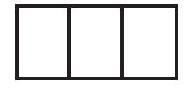
\includegraphics[max width=\textwidth, center]{2024_11_21_724abc2cf5a71562f5b2g-01(1)}

KOD ZDAJĄCEGO

PESEL ZDAJĄCEGO

LISTOPAD\\
2018

Wpisuje zdający przed rozpoczęciem pracy\\
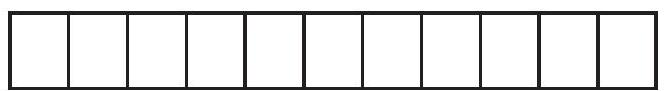
\includegraphics[max width=\textwidth, center]{2024_11_21_724abc2cf5a71562f5b2g-01}

\section*{ZADANIA ZAMKNIĘTE}
W zadaniach 1.-24. wybierz i zaznacz jedną poprawną odpowiedź.

\section*{Zadanie 1. (0-1)}
Wynikiem działania \(49^{-6}: 7^{-15}\) jest:\\
A. \(7^{-21}\)\\
B. \(7^{3}\)\\
C. \(7^{8}\)\\
D. \(7^{-27}\)

Zadanie 2. (0-1)\\
Wyrażenie \(\log _{3}(\log 30-\log 3)\) jest równe:\\
A. \(\log _{3} 10\)\\
B. 0\\
C. 1\\
D. 3

\section*{Zadanie 3. (0-1)}
Liczbą odwrotną do liczby \(\frac{\sqrt{6}-3}{3}\) jest:\\
A. \(\frac{3-\sqrt{6}}{3}\)\\
B. \(-\sqrt{6}-3\)\\
C. \(3+\sqrt{6}\)\\
D. \(\frac{\sqrt{6}+3}{5}\)

\section*{Zadanie 4. (0-1)}
Urząd skarbowy został zobowiązany do zwrotu podatku w wysokości 235,40 zł. Kwotę tę zaokrąglono do pełnych dziesiątek złotych. Błąd względny tego zaokrąglenia wyrażony w procentach wyniósł około:\\
A. \(0,04 \%\)\\
B. \(1,95 \%\)\\
C. \(1,92 \%\)\\
D. \(2,29 \%\)

\section*{Zadanie 5. (0-1)}
Liczba \(2-2(\sqrt{3}-1)^{2}\) :\\
A. należy do przedziału \(\langle 1 ;+\infty)\)\\
B. jest ujemna\\
C. jest równa 0\\
D. należy do przedziału \((0 ; 1)\)

\section*{Zadanie 6. (0-1)}
Nierówność \(\frac{1}{3}-\frac{1}{2} x<\frac{1}{6}\) jest równoważna nierówności:\\
A. \(x>\frac{1}{3}\)\\
B. \(x<\frac{1}{3}\)\\
C. \(x>3\)\\
D. \(x<3\)

\section*{Zadanie 7. (0-1)}
Liczba różnych rozwiązań równania \(\frac{3 x\left(x^{2}-9\right)}{x-3}=0\) wynosi:\\
A. 4\\
B. 3\\
C. 2\\
D. 1

BRUDNOPIS (nie podlega ocenie)\\

\includegraphics[max width=\textwidth, center]{2024_11_21_724abc2cf5a71562f5b2g-03}

\section*{Zadanie 8. (0-1)}
Na rysunku przedstawiono wykres pewnej funkcji \(f\). Maksymalny przedział, w którym funkcja \(f\) jest rosnąca, to:\\
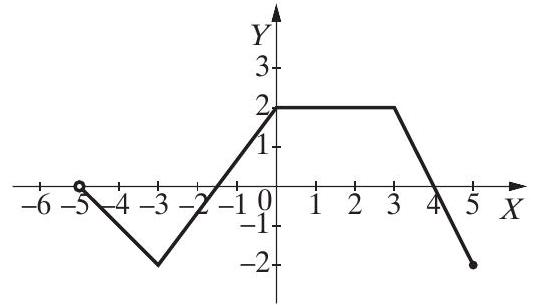
\includegraphics[max width=\textwidth, center]{2024_11_21_724abc2cf5a71562f5b2g-04}\\
A. \(\langle-2 ; 0\rangle\)\\
B. \(\langle-2 ; 2\rangle\)\\
C. \(\langle-3 ; 2\rangle\)\\
D. \(\langle-3 ; 0\rangle\)

\section*{Zadanie 9. (0-1)}
Wykres funkcji liniowej \(f(x)=\frac{8-3 x}{2}\) przecina osie układu współrzędnych w punktach \(A\) i \(B\). Pole trójkąta \(A B O\), w którym punkt \(O\) jest początkiem układu współrzędnych, wynosi:\\
A. \(10 \frac{2}{3}\)\\
B. \(5 \frac{1}{3}\)\\
C. \(21 \frac{1}{3}\)\\
D. \(7 \frac{1}{2}\)

Zadanie 10. (0-1)\\
Zbiorem wartości funkcji \(f(x)=-(x+7)(x-3)\) jest:\\
A. \((-\infty ; 25\rangle\)\\
B. \((-\infty ;-2\rangle\)\\
C. \(\langle 25 ;+\infty)\)\\
D. \(\left(-\infty ; 2 \frac{1}{2}\right)\)

\section*{Zadanie 11. (0-1)}
Wykres funkcji \(f(x)=-3^{x}\) przesunięto równolegle wzdłuż osi \(O X\) o dwie jednostki w prawo i otrzymano wykres funkcji \(y=g(x)\). Wówczas:\\
A. \(g(x)=-3^{x}+2\)\\
B. \(g(x)=-3^{x+2}\)\\
C. \(g(x)=-3^{x}-2\)\\
D. \(g(x)=-3^{x-2}\)

\section*{Zadanie 12. (0-1)}
Dodatnich wyrazów ciągu określonego wzorem \(a_{n}=-2 n+2018\) dla \(n \geq 1\) jest:\\
A. nieskończenie wiele\\
B. 1009\\
C. 1008\\
D. 2016

\section*{Zadanie 13. (0-1)}
Sumę \(n\) początkowych wyrazów ciągu \((4,6,9, \ldots)\) można obliczyć ze wzoru:\\
A. \(n(n+3)\)\\
B. \(\frac{3 n+5}{2} \cdot n\)\\
C. \(8\left[\left(\frac{3}{2}\right)^{n}-1\right]\)\\
D. \(2\left[\left(\frac{3}{2}\right)^{n}-1\right]\)

\section*{Zadanie 14. (0-1)}
W pewnym ciągu arytmetycznym suma dwóch pierwszych wyrazów jest równa \(5 \frac{1}{2}\), a suma trzech pierwszych wyrazów jest równa 12. Pierwszy wyraz tego ciągu jest równy:\\
A. \(1 \frac{1}{2}\)\\
B. \(4 \frac{1}{2}\)\\
C. \(-\frac{1}{2}\)\\
D. 1

BRUDNOPIS (nie podlega ocenie)\\

\includegraphics[max width=\textwidth, center]{2024_11_21_724abc2cf5a71562f5b2g-05}

\section*{Zadanie 15. (0-1)}
Dla pewnego kąta wypukłego \(\alpha\) mamy \(\operatorname{tg} \frac{\alpha}{3}=\frac{\sqrt{3}}{3}\). Kąt \(\alpha\) ma miarę:\\
A. \(210^{\circ}\)\\
B. \(60^{\circ}\)\\
C. \(90^{\circ}\)\\
D. \(120^{\circ}\)

\section*{Zadanie 16. (0-1)}
Wysokość rombu jest równa 12, a jego pole jest równe 180. Sinus kąta ostrego rombu wynosi:\\
A. 0,4\\
B. 0,6\\
C. 0,75\\
D. 0,8

\section*{Zadanie 17. (0-1)}
Punkty \(A, B, C\) i \(D\) należą do okręgu o środku w punkcie \(O\) (patrz rys.). Suma \(\alpha+\beta\) wynosi:\\
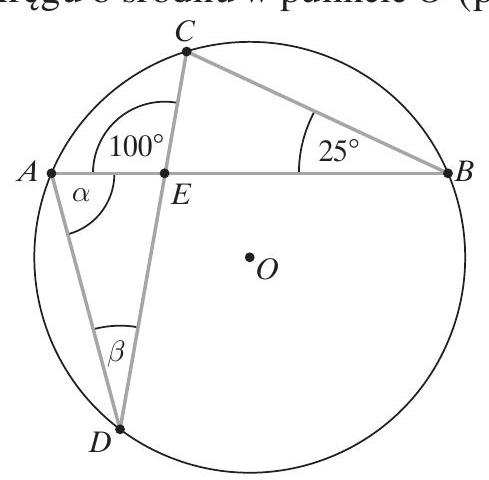
\includegraphics[max width=\textwidth, center]{2024_11_21_724abc2cf5a71562f5b2g-06}\\
A. \(125^{\circ}\)\\
B. \(120^{\circ}\)\\
C. \(100^{\circ}\)\\
D. \(90^{\circ}\)

\section*{Zadanie 18. (0-1)}
Obserwowana w laboratorium populacja bakterii podwaja swoją liczebność co 20 minut. Początkowa liczba bakterii wynosiła \(K\) sztuk. Oznacza to, że po upływie \(n\) godzin liczebność populacji wyniesie:\\
A. \(K \cdot 2^{3 n}\)\\
B. \(K \cdot 6^{n}\)\\
C. \(K^{3 n}\)\\
D. \(K \cdot 3 n\)

\section*{Zadanie 19. (0-1)}
Przeciwległe wierzchołki kwadratu mają współrzędne \(A=(1,-3)\) i \(C=(-5,3)\). Bok kwadratu ma długość:\\
A. 12\\
B. \(6 \sqrt{2}\)\\
C. \(3 \sqrt{2}\)\\
D. 6

\section*{Zadanie 20. (0-1)}
Ilość wszystkich liczb czterocyfrowych, w których cyfry się nie powtarzają, wynosi:\\
A. 9.9.8.7\\
B. \(10 \cdot 9 \cdot 8 \cdot 7\)\\
C. 9•10 • 10 • 10\\
D. \(9 \cdot 8 \cdot 7 \cdot 6\)

Zadanie 21. (0-1)\\
Rzucono trzy razy monetą symetryczną. Prawdopodobieństwo uzyskania jednej reszki wynosi:\\
A. \(\frac{1}{2}\)\\
B. \(\frac{3}{8}\)\\
C. \(\frac{7}{8}\)\\
D. \(\frac{1}{8}\)

BRUDNOPIS (nie podlega ocenie)\\

\includegraphics[max width=\textwidth, center]{2024_11_21_724abc2cf5a71562f5b2g-07}

\section*{Zadanie 22. (0-1)}
Średnia arytmetyczna zestawu liczb 5, 8, 1, 3, x, 8 wynosi 6 . Mediana tego zestawu jest równa:\\
A. 2\\
B. \(6 \frac{1}{2}\)\\
C. 4\\
D. 8

\section*{Zadanie 23. (0-1)}
Na rysunku przedstawiono graniastosłup prawidłowy czworokątny o krawędzi podstawy równej 4. Graniastosłup ten przecięto płaszczyzną przechodzącą przez przekątną \(B D\) podstawy i wierzchołek \(C^{\prime}\). Otrzymany przekrój jest trójkątem, którego wysokość poprowadzona z wierzchołka \(C^{\prime}\) jest równa 12. Wysokość graniastosłupa jest równa:\\
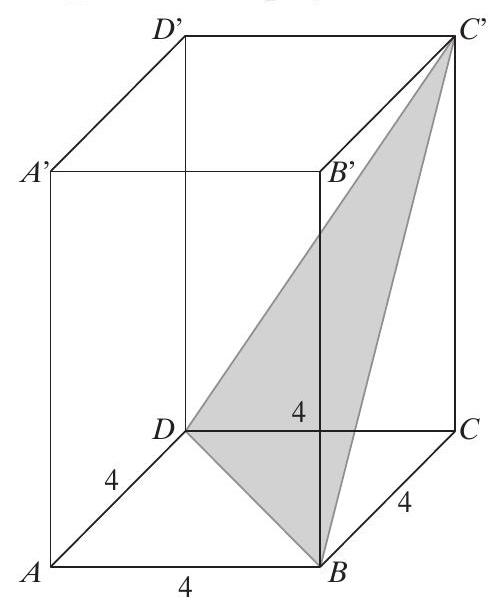
\includegraphics[max width=\textwidth, center]{2024_11_21_724abc2cf5a71562f5b2g-08}\\
A. \(2 \sqrt{35}\)\\
B. \(4 \sqrt{7}\)\\
C. \(2 \sqrt{34}\)\\
D. \(8 \sqrt{2}\)

\section*{Zadanie 24. (0-1)}
Kula o promieniu 6 cm i walec o wysokości równej \(4,5 \mathrm{~cm}\) mają równe objętości. Średnica podstawy walca ma długość:\\
A. 8 cm\\
B. \(8 \sqrt{2} \mathrm{~cm}\)\\
C. 16 cm\\
D. 20 cm

BRUDNOPIS (nie podlega ocenie)\\

\includegraphics[max width=\textwidth, center]{2024_11_21_724abc2cf5a71562f5b2g-09}

\section*{ZADANIA OTWARTE}
Rozwiązania zadań 25.-34. należy zapisać w wyznaczonych miejscach pod treścią zadania.

\section*{Zadanie 25. (0-2)}
Rozwiąż nierówność \((2 x-5)(3-x)>-66\).\\

\includegraphics[max width=\textwidth, center]{2024_11_21_724abc2cf5a71562f5b2g-10}

Odpowiedź:

\section*{Zadanie 26. (0-2)}
W trapezie \(A B C D\) przekątne przecinają się w punkcie \(P\). Punkt \(P\) dzieli przekątne na odcinki długości: \(|A P|=8,|P C|=3\) i \(|B P|=12\). Długości podstaw \(A B\) i \(C D\) trapezu różnią się o 15 . Oblicz długość odcinka \(D P\) oraz długości podstaw \(A B\) i \(C D\) trapezu.\\
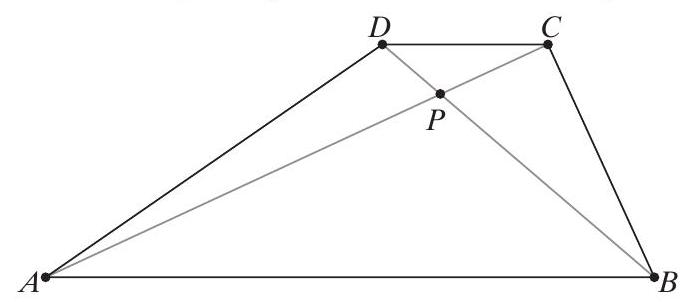
\includegraphics[max width=\textwidth, center]{2024_11_21_724abc2cf5a71562f5b2g-10(1)}

\begin{center}
\begin{tabular}{|c|c|c|c|c|c|c|c|c|c|c|c|c|c|c|c|c|c|c|c|c|c|c|}
\hline
 &  &  &  &  &  &  &  &  &  &  &  &  &  &  &  &  &  &  &  &  &  &  \\
\hline
到 &  &  &  &  &  &  &  &  &  &  &  &  &  &  &  &  &  &  &  &  &  &  \\
\hline
 &  &  &  &  &  &  &  &  &  &  &  &  &  &  &  &  &  &  &  &  &  &  \\
\hline
 &  &  &  &  &  &  &  &  &  &  &  &  &  &  &  &  &  &  &  &  &  &  \\
\hline
 &  &  &  &  &  &  &  &  &  &  &  &  &  &  &  &  &  &  &  &  &  &  \\
\hline
 &  &  &  &  &  &  &  &  &  &  &  &  &  &  &  &  &  &  &  &  &  &  \\
\hline
 &  &  &  &  &  &  &  &  &  &  &  &  &  &  &  &  &  &  &  &  &  &  \\
\hline
 &  &  &  &  &  &  &  &  &  &  &  &  &  &  &  &  &  &  &  &  &  &  \\
\hline
 &  &  &  &  &  &  &  &  &  &  &  &  &  &  &  &  &  &  &  &  &  &  \\
\hline
 &  &  &  &  &  &  &  &  &  &  &  &  &  &  &  &  &  &  &  &  &  &  \\
\hline
 &  &  &  &  &  &  &  &  &  &  &  &  &  &  &  &  &  &  &  &  &  &  \\
\hline
 &  &  &  &  &  &  &  &  &  &  &  &  &  &  &  &  &  &  &  &  &  &  \\
\hline
\end{tabular}
\end{center}

Odpowiedź: \(\qquad\)

\section*{Zadanie 27. (0-2)}
Wykaż, że jeżeli liczby \(a\) i \(b\) są kolejnymi liczbami naturalnymi, to liczba \(\left(a+\frac{1}{2} b\right)^{2}-\left(a-\frac{1}{2} b\right)^{2}\)\\
jest podzielna przez 4.\\

\includegraphics[max width=\textwidth, center]{2024_11_21_724abc2cf5a71562f5b2g-11}

\section*{Zadanie 28. (0-2)}
Wiedząc, że kąt \(\alpha\) jest rozwarty oraz \(\sin ^{2} \alpha=\frac{9}{25}\), oblicz \(\operatorname{tg} \alpha\).

\begin{center}
\begin{tabular}{|c|c|c|c|c|c|c|c|c|c|c|c|c|c|c|c|c|c|c|c|c|c|}
\hline
 &  &  &  &  &  &  &  &  &  &  &  &  &  &  &  &  &  &  &  &  &  \\
\hline
 &  &  &  &  &  &  &  &  &  &  &  &  &  &  &  &  &  &  &  &  &  \\
\hline
 &  &  &  &  &  &  &  &  &  &  &  &  &  &  &  &  &  &  &  &  &  \\
\hline
 &  &  &  &  &  &  &  &  &  &  &  &  &  &  &  &  &  &  &  &  &  \\
\hline
 &  &  &  &  &  &  &  &  &  &  &  &  &  &  &  &  &  &  &  &  &  \\
\hline
 &  &  &  &  &  &  &  &  &  &  &  &  &  &  &  &  &  &  &  &  &  \\
\hline
 &  &  &  &  &  &  &  &  &  &  &  &  &  &  &  &  &  &  &  &  &  \\
\hline
 &  &  &  &  &  &  &  &  &  &  &  &  &  &  &  &  &  &  &  &  &  \\
\hline
 &  &  &  &  &  &  &  &  &  &  &  &  &  &  &  &  &  &  &  &  &  \\
\hline
 &  &  &  &  &  &  &  &  &  &  &  &  &  &  &  &  &  &  &  &  &  \\
\hline
 &  &  &  &  &  &  &  &  &  &  &  &  &  &  &  &  &  &  &  &  &  \\
\hline
 &  &  &  &  &  &  &  &  &  &  &  &  &  &  &  &  &  &  &  &  &  \\
\hline
 &  &  &  &  &  &  &  &  &  &  &  &  &  &  &  &  &  &  &  &  &  \\
\hline
 &  &  &  &  &  &  &  &  &  &  &  &  &  &  &  &  &  &  &  &  &  \\
\hline
 &  &  &  &  &  &  &  &  &  &  &  &  &  &  &  &  &  &  &  &  &  \\
\hline
 &  &  &  &  &  &  &  &  &  &  &  &  &  &  &  &  &  &  &  &  &  \\
\hline
 &  &  &  &  &  &  &  &  &  &  &  &  &  &  &  &  &  &  &  &  &  \\
\hline
\end{tabular}
\end{center}

Odpowiedź:

\section*{Zadanie 29. (0-2)}
Dana jest funkcja \(f(x)=-3 x^{2}+b x+c\) dla \(x \in \boldsymbol{R}\). Prosta o równaniu \(x=2\) jest osią symetrii paraboli będącej jej wykresem, a zbiorem wartości funkcji \(f\) jest przedział \((-\infty ; 21\rangle\). Wyznacz współczynniki \(b\) i \(c\).\\

\includegraphics[max width=\textwidth, center]{2024_11_21_724abc2cf5a71562f5b2g-12(1)}

Odpowiedź:

\section*{Zadanie 30. (0-2)}
Do okręgu o środku w punkcie \(O\) poprowadzono z trzech punktów \(A, B\) i \(C\) leżących na okręgu styczne, które przecięły się w punktach \(D, E\) i \(F\) (zobacz rysunek). Wykaż, że jeżeli \(|A F|=x\), to obwód trójkąta \(D E F\) jest równy \(2 x\).\\
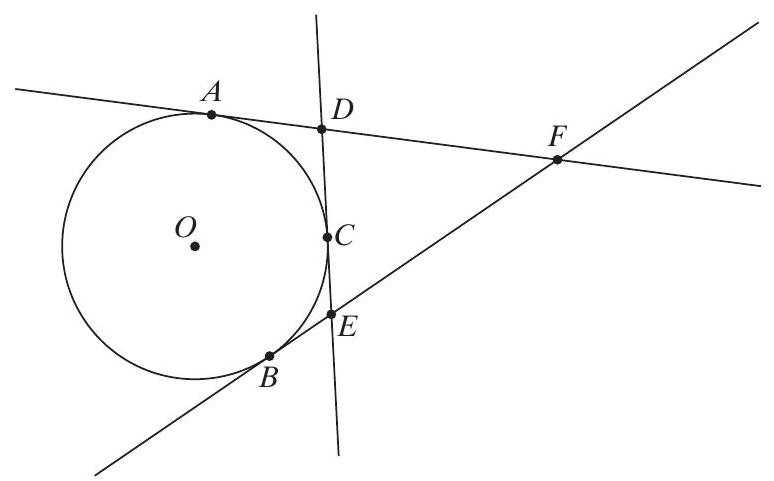
\includegraphics[max width=\textwidth, center]{2024_11_21_724abc2cf5a71562f5b2g-12}

\begin{center}
\begin{tabular}{|c|c|c|c|c|c|c|c|c|c|c|c|c|c|c|c|c|c|c|c|c|c|c|c|c|c|c|c|c|c|}
\hline
 &  &  &  &  &  &  &  &  &  &  &  &  &  &  &  &  &  &  &  &  &  &  &  &  &  &  &  &  &  \\
\hline
 &  &  &  &  &  &  &  &  &  &  &  &  &  &  &  &  &  &  &  &  &  &  &  &  &  &  &  &  &  \\
\hline
 &  &  &  &  &  &  &  &  &  &  &  &  &  &  &  &  &  &  &  &  &  &  &  &  &  &  &  &  &  \\
\hline
 &  &  &  &  &  &  &  &  &  &  &  &  &  &  &  &  &  &  &  &  &  &  &  &  &  &  &  &  &  \\
\hline
 &  &  &  &  &  &  &  &  &  &  &  &  &  &  &  &  &  &  &  &  &  &  &  &  &  &  &  &  &  \\
\hline
 &  &  &  &  &  &  &  &  &  &  &  &  &  &  &  &  &  &  &  &  &  &  &  &  &  &  &  &  &  \\
\hline
 &  &  &  &  &  &  &  &  &  &  &  &  &  &  &  &  &  &  &  &  &  &  &  &  &  &  &  &  &  \\
\hline
 &  &  &  &  &  &  &  &  &  &  &  &  &  &  &  &  &  &  &  &  &  &  &  &  &  &  &  &  &  \\
\hline
 &  &  &  &  &  &  &  &  &  &  &  &  &  &  &  &  &  &  &  &  &  &  &  &  &  &  &  &  &  \\
\hline
 &  &  &  &  &  &  &  &  &  &  &  &  &  &  &  &  &  &  &  &  &  &  &  &  &  &  &  &  &  \\
\hline
 &  &  &  &  &  &  &  &  &  &  &  &  &  &  &  &  &  &  &  &  &  &  &  &  &  &  &  &  &  \\
\hline
\end{tabular}
\end{center}

\section*{Zadanie 31. (0-2)}
Spośród wszystkich wierzchołków sześciokąta foremnego o krawędzi 1 losujemy dowolne dwa. Oblicz prawdopodobieństwo tego, że wylosowane wierzchołki utworzą odcinek, którego długość jest liczbą niewymierną.

\begin{center}
\begin{tabular}{|c|c|c|c|c|c|c|c|c|c|c|c|c|c|c|c|c|c|c|c|c|}
\hline
 &  &  &  &  &  &  &  &  &  &  &  &  &  &  &  &  &  &  &  &  \\
\hline
 &  &  &  &  &  &  &  &  &  &  &  &  &  &  &  &  &  &  &  &  \\
\hline
 &  &  &  &  &  &  &  &  &  &  &  &  &  &  &  &  &  &  &  &  \\
\hline
 &  &  &  &  &  &  &  &  &  &  &  & 到 &  & - &  & 到 &  &  &  &  \\
\hline
 &  &  &  &  &  &  &  &  &  &  &  &  &  &  &  &  &  &  &  &  \\
\hline
 &  &  &  &  &  &  &  &  &  &  &  &  &  &  &  &  &  &  &  &  \\
\hline
 &  &  &  &  &  &  &  &  &  &  &  &  &  &  &  &  &  &  &  &  \\
\hline
 &  &  &  &  &  &  &  &  &  &  &  &  &  &  &  &  &  &  &  &  \\
\hline
 &  &  &  &  &  &  &  &  &  &  &  &  &  &  &  &  &  &  &  &  \\
\hline
 &  &  &  &  &  &  &  &  &  &  &  &  &  &  &  &  &  &  &  &  \\
\hline
 &  &  &  &  &  &  &  &  &  &  &  &  &  &  &  &  &  &  &  &  \\
\hline
 &  &  &  &  &  &  &  &  &  &  &  &  &  &  &  &  &  &  &  &  \\
\hline
 &  &  &  &  &  &  &  &  &  &  &  &  &  &  &  &  &  &  &  &  \\
\hline
 &  &  &  &  &  &  &  &  &  &  &  &  &  &  &  &  &  &  &  &  \\
\hline
\end{tabular}
\end{center}

Odpowiedź: \(\qquad\)

\section*{Zadanie 32. (0-3)}
Dany jest skónczony, pięciowyrazowy ciąg \((4 a-5 ; a ; b ; b+2 ; 9)\). Trzy pierwsze wyrazy tego ciągu są trzema kolejnymi wyrazami ciągu arytmetycznego, a trzy ostatnie są trzema kolejnymi wyrazami ciągu geometrycznego. Oblicz \(a\) i \(b\).

\begin{center}
\begin{tabular}{|c|c|c|c|c|c|c|c|c|c|c|c|c|c|c|c|c|c|c|c|c|c|c|}
\hline
 &  &  &  &  &  &  &  &  &  &  &  &  &  &  &  &  &  &  &  &  &  &  \\
\hline
 &  &  &  &  &  &  &  &  &  &  &  &  &  &  &  &  &  &  &  &  &  &  \\
\hline
 &  &  &  &  &  &  &  &  &  &  &  &  &  &  &  &  &  &  &  &  &  &  \\
\hline
 &  &  &  &  &  &  &  &  &  &  &  &  &  &  &  &  &  &  &  &  &  &  \\
\hline
 &  &  &  &  &  &  &  &  &  &  &  &  &  &  &  &  &  &  &  &  &  &  \\
\hline
 &  &  &  &  &  &  &  &  &  &  &  &  &  &  &  &  &  &  &  &  &  &  \\
\hline
 &  &  &  &  &  &  &  &  &  &  &  &  &  &  &  &  &  &  &  &  &  &  \\
\hline
 &  &  &  &  &  &  &  &  &  &  &  &  &  &  &  &  &  &  &  &  &  &  \\
\hline
 &  &  &  &  &  &  &  &  &  &  &  &  &  &  &  &  &  &  &  &  &  &  \\
\hline
 &  &  &  &  &  &  &  &  &  &  &  &  &  &  &  &  &  &  &  &  &  &  \\
\hline
 &  &  &  &  &  &  &  &  &  &  &  &  &  &  &  &  &  &  &  &  &  &  \\
\hline
 &  &  &  &  &  &  &  &  &  &  &  &  &  &  &  &  &  &  &  &  &  &  \\
\hline
 &  &  &  &  &  &  &  &  &  &  &  &  &  &  &  &  &  &  &  &  &  &  \\
\hline
 &  &  &  &  &  &  &  &  &  &  &  &  &  &  &  &  &  &  &  &  &  &  \\
\hline
 &  &  &  &  &  &  &  &  &  &  &  &  &  &  &  &  &  &  &  &  &  &  \\
\hline
 &  &  &  &  &  &  &  &  &  &  &  &  &  &  &  &  &  &  &  &  &  &  \\
\hline
 &  &  &  &  &  &  &  &  &  &  &  &  &  &  &  &  &  &  &  &  &  &  \\
\hline
 &  &  &  &  &  &  &  &  &  &  &  &  &  &  &  &  &  &  &  &  &  &  \\
\hline
\end{tabular}
\end{center}

Odpowiedź: \(\qquad\)

\section*{Zadanie 33. (0-4)}
Dany jest trójkąt \(A B C\), w którym \(A=(-9,8)\). Bok \(B C\) tego trójkąta zawiera się w prostej o równaniu \(y=-2 x+38\). Prosta zawierająca wysokość tego trójkąta poprowadzona z wierzchołka \(B\) ma równanie \(3 x+2 y-61=0\). Wyznacz współrzędne wierzchołków \(B\) i \(C\) oraz napisz równanie prostej zawierającej wysokość trójkąta poprowadzoną z wierzchołka \(C\).\\

\includegraphics[max width=\textwidth, center]{2024_11_21_724abc2cf5a71562f5b2g-14}

Odpowiedź:

\section*{Zadanie 34. (0-5)}
W ostrosłupie prawidłowym trójkątnym krawędź boczna jest trzy razy dłuższa od wysokości ostrosłupa. Krawędź podstawy ma długość 12. Oblicz objętość i pole powierzchni bocznej tego ostrosłupa.

\begin{center}
\begin{tabular}{|c|c|c|c|c|c|c|c|c|c|c|c|c|c|c|c|c|c|c|c|c|}
\hline
 &  &  &  &  &  &  &  &  &  &  &  &  &  &  &  &  &  &  &  &  \\
\hline
 &  &  &  &  &  &  &  &  &  &  &  &  &  &  &  &  &  &  &  &  \\
\hline
 &  &  &  &  &  &  &  &  &  &  &  &  &  &  &  &  &  &  &  &  \\
\hline
 &  &  &  &  &  &  &  &  &  &  &  &  &  &  &  &  &  &  &  &  \\
\hline
 &  &  &  &  &  &  &  &  &  &  &  &  &  &  &  &  &  &  &  &  \\
\hline
 &  &  &  &  &  &  &  &  &  &  &  &  &  &  &  &  &  &  &  &  \\
\hline
 &  &  &  &  &  &  &  &  &  &  &  &  &  &  &  &  &  &  &  &  \\
\hline
 &  &  &  &  &  &  &  &  &  &  &  &  &  &  &  &  &  &  &  &  \\
\hline
 &  &  &  &  &  &  &  &  &  &  &  &  &  &  &  &  &  &  &  &  \\
\hline
 &  &  &  &  &  &  &  &  &  &  &  &  &  &  &  &  &  &  &  &  \\
\hline
 &  &  &  &  &  &  &  &  &  &  &  &  &  &  &  &  &  &  &  &  \\
\hline
 &  &  &  &  &  &  &  &  &  &  &  &  &  &  &  &  &  &  &  &  \\
\hline
 &  &  &  &  &  &  &  &  &  &  &  &  &  &  &  &  &  &  &  &  \\
\hline
 &  &  &  &  &  &  &  &  &  &  &  &  &  &  &  &  &  &  &  &  \\
\hline
 &  &  &  &  &  &  &  &  &  &  &  &  &  &  &  &  &  &  &  &  \\
\hline
 &  &  &  &  &  &  &  &  &  &  &  &  &  &  &  &  &  &  &  &  \\
\hline
 &  &  &  &  &  &  &  &  &  &  &  &  &  &  &  &  &  &  &  &  \\
\hline
 &  &  &  &  &  &  &  &  &  &  &  &  &  &  &  &  &  &  &  &  \\
\hline
 &  &  &  &  &  &  &  &  &  &  &  &  &  &  &  &  &  &  &  &  \\
\hline
 &  &  &  &  &  &  &  &  &  &  &  &  &  &  &  &  &  &  &  &  \\
\hline
 &  &  &  &  &  &  &  &  &  &  &  &  &  &  &  &  &  &  &  &  \\
\hline
 &  &  &  &  &  &  &  &  &  &  &  &  &  &  &  &  &  &  &  &  \\
\hline
 &  &  &  &  &  &  &  &  &  &  &  &  &  &  &  &  &  &  &  &  \\
\hline
 &  &  &  &  &  &  &  &  &  &  &  &  &  &  &  &  &  &  &  &  \\
\hline
 &  &  &  &  &  &  &  &  &  &  &  &  &  &  &  &  &  &  &  &  \\
\hline
 &  &  &  &  &  &  &  &  &  &  &  &  &  &  &  &  &  &  &  &  \\
\hline
 &  &  &  &  &  &  &  &  &  &  &  &  &  &  &  &  &  &  &  &  \\
\hline
 &  &  &  &  &  &  &  &  &  &  &  &  &  &  &  &  &  &  &  &  \\
\hline
 &  &  &  &  &  &  &  &  &  &  &  &  &  &  &  &  &  &  &  &  \\
\hline
 &  &  &  &  &  &  &  &  &  &  &  &  &  &  &  &  &  &  &  &  \\
\hline
 &  &  &  &  &  &  &  &  &  &  &  &  &  &  &  &  &  &  &  &  \\
\hline
 &  &  &  &  &  &  &  &  &  &  &  &  &  &  &  &  &  &  &  &  \\
\hline
 &  &  &  &  &  &  &  &  &  &  &  &  &  &  &  &  &  &  &  &  \\
\hline
 &  &  &  &  &  &  &  &  &  &  &  &  &  &  &  &  &  &  &  &  \\
\hline
 &  &  &  &  &  &  &  &  &  &  &  &  &  &  &  &  &  &  &  &  \\
\hline
 &  &  &  &  &  &  &  &  &  &  &  &  &  &  &  &  &  &  &  &  \\
\hline
 &  &  &  &  &  &  &  &  &  &  &  &  &  &  &  &  &  &  &  &  \\
\hline
 &  &  &  &  &  &  &  &  &  &  &  &  &  &  &  &  &  &  &  &  \\
\hline
 &  &  &  &  &  &  &  &  &  &  &  &  &  &  &  &  &  &  &  &  \\
\hline
 &  &  &  &  &  &  &  &  &  &  &  &  &  &  &  &  &  &  &  &  \\
\hline
\end{tabular}
\end{center}

Odpowiedź:

\section*{BRUDNOPIS (nie podlega ocenie)}
\begin{center}

\includegraphics[max width=\textwidth]{2024_11_21_724abc2cf5a71562f5b2g-16}
\end{center}


\end{document}